\documentclass[screen, aspectratio=43]{beamer}
\usepackage[T1]{fontenc}
\usepackage[utf8]{inputenc}

% Use the NTNU-temaet for beamer 
% \usetheme[style=ntnu|simple|vertical|horizontal, 
%     language=bm|nn|en, 
%     smalltitle, 
%     city=all|trondheim|alesund|gjovik]{ntnu2017}
\usetheme[style=ntnu, language=en, smalltitle]{ntnu2017}

\usepackage[english]{babel}
\usepackage[style=numeric,backend=biber,natbib=false,sorting=none]{biblatex}

\title[PCW-d1]{Physical Computing Workshop: Day 3}
%\subtitle{Microcontrollers, APIs, sonification, and big data}
\subtitle{Embedded Sensors and Actuators}
\author[A. Xamb{\'o}]{Anna Xamb{\'o}}
\institute[NTNU]{Department of Music, NTNU}
\date{17 October 2019}
%\date{} % To have an empty date

\addbibresource{../pcw.bib} % Add bibliography database

% Set the reference style to numeric.
% See here: http://tex.stackexchange.com/questions/68080/beamer-bibliography-icon
\setbeamertemplate{bibliography item}[text] 

% Set bibliography fonts to a small size.
\renewcommand*{\bibfont}{\footnotesize}

\begin{document}

\begin{frame}
  \titlepage
\end{frame}
%
\begin{frame}
\frametitle{The MCT4045 Bela Kit}
       \begin{figure}
	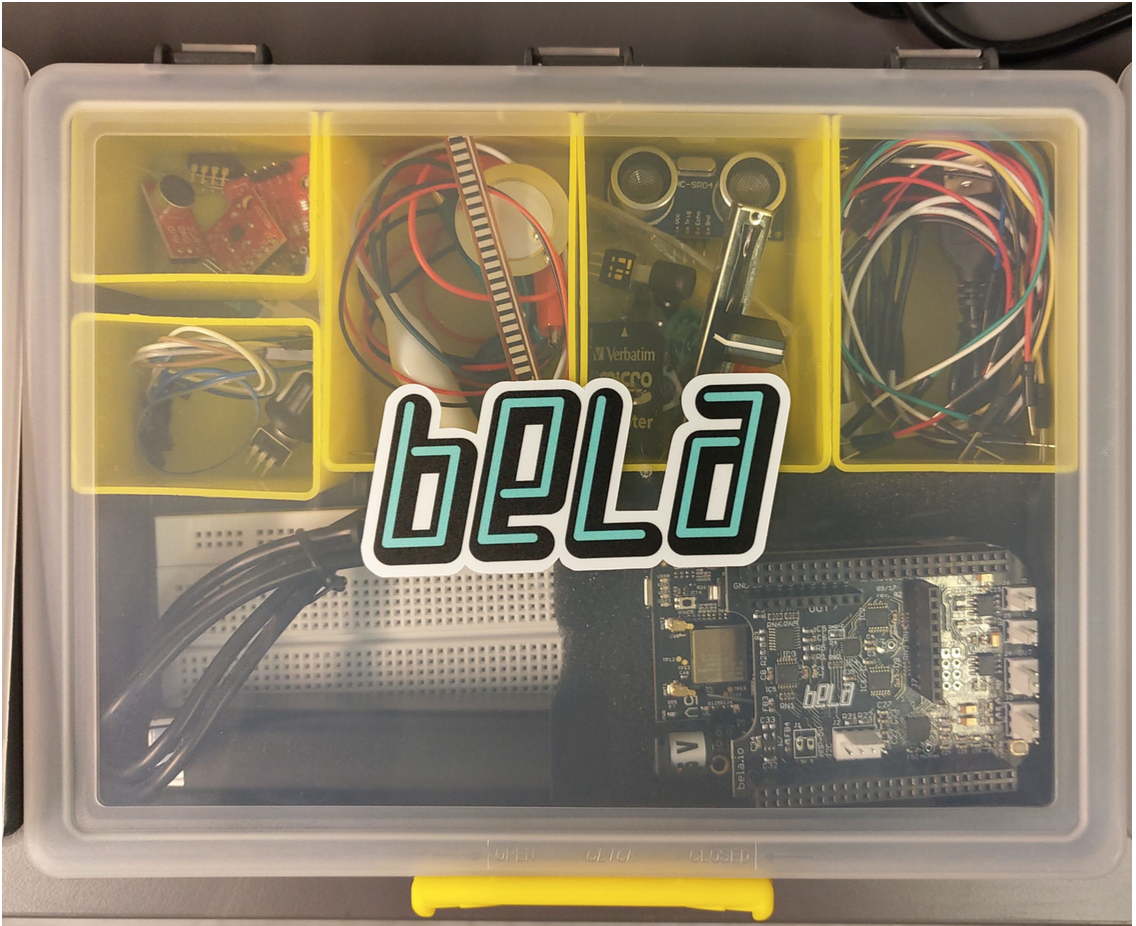
\includegraphics[scale=0.25]{img/Bela-kit.png}
	\end{figure}
\begin{itemize}
\item Kit designed by Stefano Fasciani for the course MCT4045 (scheduled in the 3rd semester of MCT).
\item Technical details and datasheet of all parts included in the MCT Hardware Kit are available at:\\ 
\url{https://uio.instructure.com/courses/22318/files/503966/download?wrap=1}
\end{itemize}
\end{frame}
%
\usebackgroundtemplate{}
\begin{frame}
\frametitle{Warm-up Activity\\How would I map from \dots to \dots?}
Pick one component from the MCT Bela hardware kit and explain it to the class in terms of:
\begin{itemize}
\item Characteristics of the component
\item Potential mapping to an interactive music system e.g. what audio/music parameter would you modify/control?
\end{itemize}
\end{frame}
%
\begin{frame}
\frametitle{Learning Outcomes}
By the end of the session,  you will be able to...
\begin{itemize}
\item Identify the basic differences between sensors and actuators.
\item Get a sense of the main parts when designing an interactive system.
\item Be exposed to real-world projects based on physical computing.
\item Discern the differences between digital and analog sensors and actuators.
\item Be able to normalize sensor data.
\item Explore mappings from sensor data to sound.
\item Demonstrate a custom-made musical instrument in a performance setting.
\end{itemize}
\end{frame}
%
\usebackgroundtemplate{}
\begin{frame}
\frametitle{}
{\huge Physical Computing: Sensors and Actuators}
\end{frame}
%
\begin{frame}
\frametitle{Physical Computing}
\begin{itemize}
\item Physical computing involves the communication between our physical world and the digital world of computers.
\item The way this is made possible is through the process of transduction, which is the conversion of one form of energy to another.
\item The use of microcontrollers can provide vast opportunities to develop reactive and interactive sound projects beyond using a computer keyboard, mouse, screen and speakers.
\item The types of inputs and outputs that are available to use to make transduction possible and how to process the data.
\end{itemize}
{\tiny
Nazemi, M. (2019). Sonic Interaction With Physical Computing. Foundations in Sound Design for Embedded Media: A Multidisciplinary Approach. \cite{Nazemi.2019.SID}
}	
\end{frame}
%
\begin{frame}
\frametitle{Input}
\begin{itemize}
\item Inputs can be sensors, switches, levers or sliders.
\item Sensors: There are two broad categories of sensors, digital (number of states, usually 2) or analog (continuous range of states). 
\item The use of microcontrollers can provide vast opportunities to develop reactive and interactive sound projects beyond using a computer keyboard, mouse, screen and speakers.
\item There is a range of sensors available: \emph{sensing pressure} (e.g. force resistive sensor (FSR)), \emph{sensing the environment} (e.g. temperature, photoresistors), \emph{sensing movement/distance} (e.g. accelerometer, gyroscope), \emph{sensing body} (e.g., muscle Sensor (EMG), brain waves (EEG)).
\end{itemize}
{\tiny
Nazemi, M. (2019). Sonic Interaction With Physical Computing. Foundations in Sound Design for Embedded Media: A Multidisciplinary Approach. \cite{Nazemi.2019.SID}
}	
\end{frame}
%
\begin{frame}
\frametitle{Output}
\begin{itemize}
\item The output is the mechanism that provides feedback to the user using movements like actuators and motors, light, video or sound. 
\end{itemize}
{\tiny
Nazemi, M. (2019). Sonic Interaction With Physical Computing. Foundations in Sound Design for Embedded Media: A Multidisciplinary Approach. \cite{Nazemi.2019.SID}
}	
\end{frame}
%
\begin{frame}
\frametitle{Processing}
\begin{itemize}
\item It requires a computer to take the information from the input, make some decisions based on changes that may occur in real time and output feedback to either the user or another computer. 
\item We need to use software to make sense of the incoming data from the input and convert that data into meaningful information to be sent out as an output for the user or as a message to another computer. 
\end{itemize}
%
{\tiny
Nazemi, M. (2019). Sonic Interaction With Physical Computing. Foundations in Sound Design for Embedded Media: A Multidisciplinary Approach. \cite{Nazemi.2019.SID}
}	
%
\end{frame}
\begin{frame}
\frametitle{Diagram of an Interactive System}
       \begin{figure}
	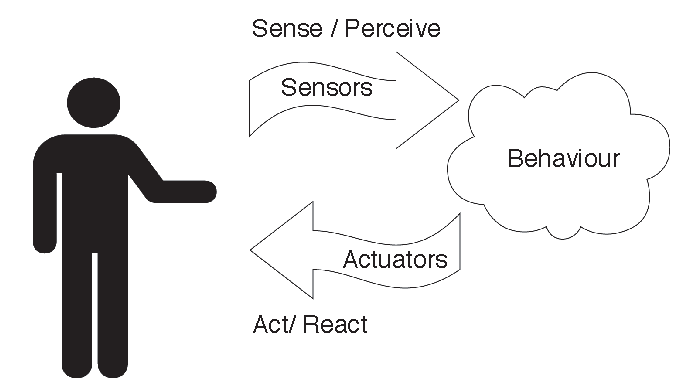
\includegraphics[scale=0.65]{img/Diagram-Banzi.pdf}
	\end{figure}
{\tiny
Banzi, M. (2009). Getting Started with Arduino. O?Reilly Media/Make.  \cite{Banzi.2009.arduino}
}	
\end{frame}
%
\begin{frame}
\frametitle{When Designing your Interactive System...}
       \begin{figure}
	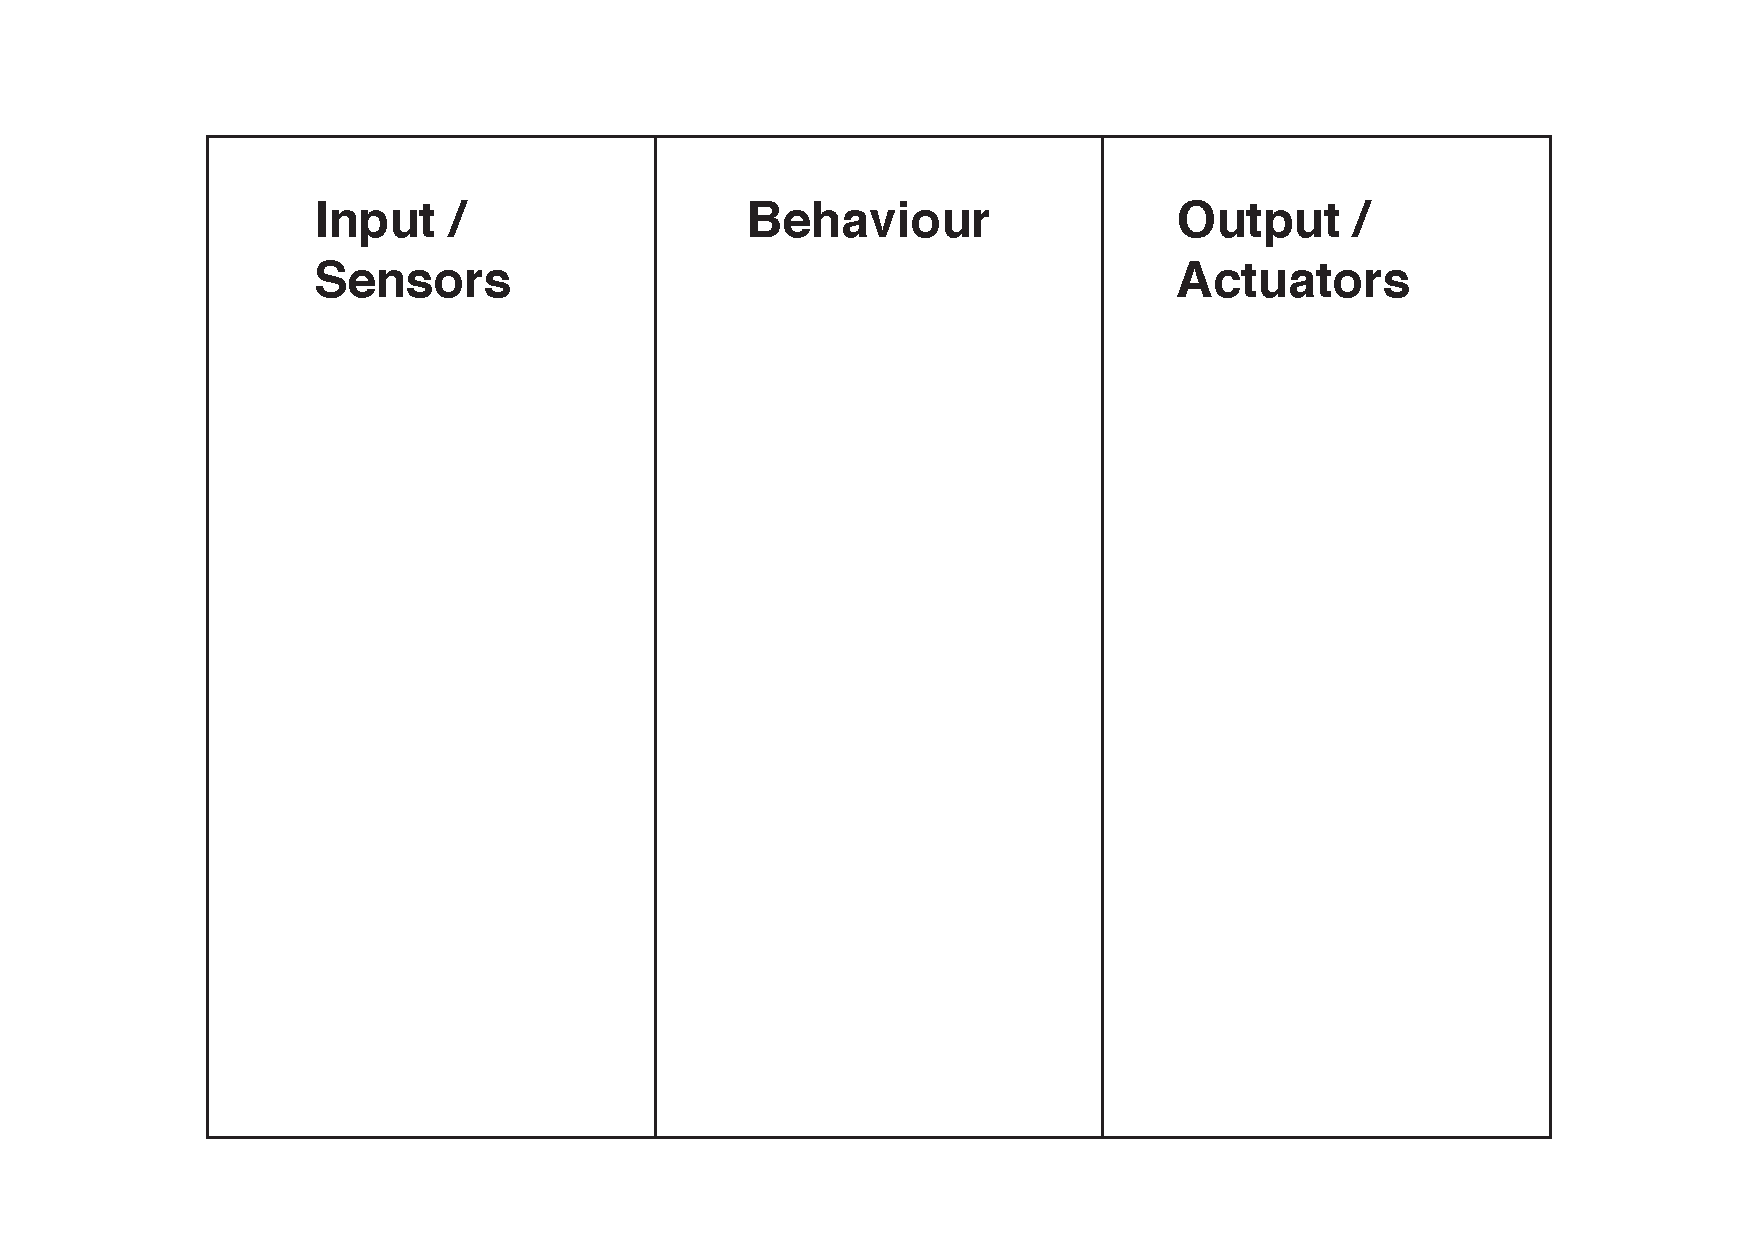
\includegraphics[scale=0.35]{img/diagram-physical-computing-system.pdf}
	\end{figure}
\end{frame}
%
\usebackgroundtemplate{}
\begin{frame}
\frametitle{}
{\huge Examples of Projects}
\end{frame}
%
%\begin{frame}
%\frametitle{Project 1:}
%\begin{itemize}
%\item  
%\end{itemize}
%{\tiny
%Ref \cite{Nazemi.2019.SID}
%}	
%\end{frame}
%
\begin{frame}
\frametitle{Project 1: Embodied Interactions}
\begin{itemize}
\item  \url{https://www.audiocommons.org/2018/05/18/tei-2018.html}
\end{itemize}
{\tiny Sophie Skach, Anna Xambo, Luca Turchet, Ariane Stolfi, Rebecca Stewart, Mathieu Barthet (2018). Embodied Interactions with E-Textiles and the Internet of Sounds for Performing Arts Proceedings of the Twelfth International Conference on Tangible, Embedded, and Embodied Interaction \cite{Skach.2018.embodied}}
%{\tiny
%Sophie Skach, Anna Xamb�, Luca Turchet, Ariane Stolfi, Rebecca Stewart, Mathieu Barthet (2018). Embodied Interactions with E-Textiles and the Internet of Sounds for Performing Arts Proceedings of the Twelfth International Conference on Tangible, Embedded, and Embodied Interaction \cite{Skach.2018.embodied}}	
\end{frame}
%
\begin{frame}
\frametitle{Project 2:}
\begin{itemize}
\item  
\end{itemize}
{\tiny
Martin, C. P., Jensenius, A. R., and Torresen, J. (2018). Composing an ensemble standstill work for Myo and Bela. In Proceedings of the International Conference on New Interfaces for Musical Expression (pp. 196-197). Virginia Tech. \cite{martin2018composing}
}	
\end{frame}
%
\usebackgroundtemplate{}
\begin{frame}
\frametitle{}
{\huge Bela examples \& Workflow}
\end{frame}
% how to plug battery, how to load a file once connected
%
%
\begin{frame}
\frametitle{Analog vs.\ Digital}
       \begin{itemize}
     \item See code day 3
     \end{itemize}
\end{frame}
%
\begin{frame}
  \frametitle{Normalization of Sensor Data}
  {\scriptsize Normalization by scaling between 0 and 1 (feature scaling) is a common calculation to facilitate relations with other domains e.g. mappings to sound. The formula for normalization is:\\
  $x_{new} = \dfrac{x-x_{min}}{x_{max}-x_{min}}$
  where $x_{new}$ is the normalized value, $x_{min}$ and $x_{max}$ are the minimum and maximum values within a range. 
    \begin{itemize}
    	\item Typically you can create a function so that when you call the function you get as a result the normalized value: \\
	$x_{new}$ = \emph{normalize(x, x\_{max}, x\_{min})}
    \end{itemize}
    }
\end{frame}
%
%
%\begin{frame}
%\frametitle{Learning Outcomes}
%By the end of the session, you will be able to...
%\begin{itemize}
%\item 
%\\end{itemize}
%\end{frame}
%%
%\usebackgroundtemplate{}
%\begin{frame}
%\frametitle{}
%{\huge Warm-up Activity\\Yesterday's blogpost and performance }
%\end{frame}
%%
%\begin{frame}
%\frametitle{Setting up}
%\begin{itemize}
%\item
%\end{itemize}
%\end{frame}
%%
%
%\begin{frame}
%\frametitle{Schedule}
%\begin{itemize}
%\item 
%\end{itemize}
%\end{frame}
%%

%\begin{frame}
%  \frametitle{Learning Outcomes}
%  \begin{itemize}
%    \item Get an overview of the possibilities of interaction in physical computing applied to music.
%    \item Identify the main characteristics of the Arduino board.
%    \item Explore the creation of interactive systems for music using the Arduino board.    
%    %\item Get familiar with how web APIs work.
%    %\item Be able to integrate data from web APIs to an Arduino program.
%    %\item Explore mappings from big data to sound.
%    %\item Be able to adapt javascript and Arduino code to a custom-made musical instrument.   
%    \item Get familiar with the littleBits kit.
%    \item Be able to create a music patch with littleBits.
%    \item Demonstrate a custom-made musical instrument in a performance setting.
%    \item Reflect on the custom-made musical instrument and performance using a blogging style.   
%  \end{itemize}
%\end{frame}
%\begin{frame}
%  \frametitle{Preparation: Reading}
%        \begin{itemize}
%        \item Read / skim through the following article and be ready to discuss it in class:
%         \begin{itemize}
%         \item Collins, N., 2010. Interaction (chapter 6). In Introduction to Computer Music. Wiley. \\
%         \url{https://goo.gl/zor5gN}
%         \end{itemize}    
%         \end{itemize}
%\end{frame}
%%
%\begin{frame}
%  \frametitle{Preparation: What to Bring to Class?}
%        \begin{itemize}
%        \item Your own laptop.
%        \item Headphones / earplugs.
%         \end{itemize}
%\end{frame}
%%
%\begin{frame}
%  \frametitle{Preparation: What We Do Provide?}
%        \begin{itemize}
%        \item 7 Music Angel speakers for the performance per site.
%        \item 6 Arduino Kits per site.
%        \item Slides: \url{https://github.com/axambo/physical-computing-workshop/blob/master/slides/04-d3/pcw-d3.pdf}.
%        \item Code: \url{https://github.com/axambo/physical-computing-workshop/tree/master/exercises/04-d3}.
%        \item A handout: \url{https://github.com/axambo/physical-computing-workshop/blob/master/handouts/pcw-d3-handout.pdf}.        
%         \end{itemize}
%\end{frame}
%%
%\begin{frame}
%  \frametitle{Pre-knowledge Activity: Interaction}
%  Be ready to discuss topics related to interaction from the suggested reading. In a round of 1-minute per each person briefly comment:
%  \begin{itemize}
%  \item What is interaction in computer music for you?
%  \item What is your favorite input device and why.
%  \end{itemize}
%\end{frame}
%%
%\begin{frame}
%  \frametitle{Outline}
%      \begin{itemize}
%	\item Block I: Getting familiar with the Arduino board
%	%\item Block II: Basic interactive behavior activities: mappings from big data to sound
%	\item Block II: Basic interactive behavior activities: tangible bits
%	\item Block III: Rehearsal and performance
%    \end{itemize}  
%\end{frame}
%%
%\begin{frame}
%  \frametitle{Exercise 1: Arduino as an IKEA kit}
%    \begin{itemize}
%    	\item Explore the content of the Arduino experimentation kit, ideally in pairs.
%	\item Follow the initial steps of the booklet: get familiar with the components and install the Arduino IDE software (page 3 of the booklet.
%	\item Have a close look at the breadboard.r
%	\item Have a close look at the Arduino board and the types of pins.
%    \end{itemize}
%\end{frame}
%%
%\begin{frame}
%  \frametitle{Exercise 2: ``Hello, World!''}
%    \begin{itemize}
%    	\item The ``Hello, World!'' in Arduino: Blinking LED exercise: 1) run the example from Arduino IDE (File>Examples>01.Basics>Blink) blinking the built-in LED, 2) plug an LED to 13, what happens? 3) create the circuit from CIRC-01 of the Arduino Kit (pages 8--9 of the booklet), which controls an LED in the breadboard.
%    \end{itemize}
%\end{frame}
%%
%\begin{frame}
%  \frametitle{Exercise 3: The piezo electric buzzer}
%  When applying a voltage to the contact mic or piezo buzzer, it will produce an audible click, due to the two inner discs (metallic and ceramic) repel each other.
%    \begin{itemize}
%    	\item Create the circuit from CIRC-06 of the Arduino Kit (pages 18--19 of the booklet).
%	\item Run the code explained in page 7 from ``Arduino 8-bit sound generation'' (\url{https://www.elektormagazine.com/files/attachment/331}). Make sure that the pin number is correct. 
%	\item Explore different times. What happens if the delay is 1ms?
%	\item Try now the ``Bee'' program explained in page 9 of the same book.
%    \end{itemize}
%\end{frame}
%%
%\begin{frame}
%  \frametitle{Exercise 4: Playing tones}
%  Arduino cannot imitate the sinusoidal shape perfectly. However, we can produce square waves by repeatedly switching a pin HIGH and LOW. Microcontrollers work with time (as opposed to frequency). We can define a particular frequency by defining the time period.
%	$p =  \dfrac{1}{440} = 0.002272 s = 2.272 ms = 2272  \mu s$
%    \begin{itemize}
%    	\item Explore the different notes (C4--C5) provided in page 10 from ``Arduino 8-bit sound generation'' (\url{https://www.elektormagazine.com/files/attachment/331}). 
%	\item Challenge: Run the code from \url{https://www.arduino.cc/en/Tutorial/Melody} and change the melody.
%    \end{itemize}
%\end{frame}
%%
%\begin{frame}
%  \frametitle{Exercise 5 (optional): Cloud computing with Arduino and P5.js}
%  Serial communication to a web page in a browser is possible, and thus we can communicate browser-based applications with Arduino! Here are some tutorials that are informative on how to proceed towards this direction.
%    \begin{itemize}
%    	\item Asynchronous serial communication: the basics: \url{https://itp.nyu.edu/physcomp/lessons/serial-communication/serial-communication-the-basics/}
%    	\item Serial input to P5.js: \url{https://itp.nyu.edu/physcomp/labs/labs-serial-communication/lab-serial-input-to-the-p5-js-ide/}
%	\item Serial output from P5.js: \url{https://itp.nyu.edu/physcomp/labs/labs-serial-communication/lab-serial-output-from-p5-js/}
%	%\item Serial communication with Arduiino + P5.js: \url{http://www.bonder.tech/2017/10/27/serial-communication-with-arduino-p5-js/}
%	%\item Visualize live sensor data with p5js and an Arduino: \url{https://publiclab.org/notes/warren/02-08-2018/visualize-live-sensor-data-with-p5js-and-an-arduino}
%	%\item Arduino livechart: \url{https://github.com/billroy/arduino-livechart}
%    \end{itemize}
%\end{frame}
%%
%\begin{frame}
%  \frametitle{Exercise 6: Chiptunes with litteBits}
%    \begin{itemize}
%    	\item Explore the different pieces of litteBits, get familiar with the collection.
%	\item Build a music patch.
%    \end{itemize}
%\end{frame}
%%
%\begin{frame}
%  \frametitle{Resources}
%    \begin{itemize}
%    	\item How to use a breadboard:\\
%	\url{https://youtu.be/6WReFkfrUIk}
%	\item How to use a resistor:\\
%	\url{https://www.youtube.com/watch?v=GLD7AgAYqwA}
%	\item An Introduction to the Arduino:\\
%	\url{https://www.youtube.com/watch?v=CqrQmQqpHXc}
%	\item What is an Arduino? (Arduino Uno pinout diagram included): \\
%	\url{https://learn.sparkfun.com/tutorials/what-is-an-arduino/all}
%	\item Serial Output From Arduino: 
%	\url{https://vimeo.com/237203208}
%    \end{itemize}
%\end{frame}
%
%\begin{frame}
%  \frametitle{Other Resources: Listening}
%    \begin{itemize}
%    	\item Add here the performance of littleBits
%    \end{itemize}
%\end{frame}
%
%\begin{frame}
%  \frametitle{References}
%  \printbibliography
%\end{frame}

\end{document}
